\section{Complicated Company Database Schema}
\begin{figure}[H]
    \centering
    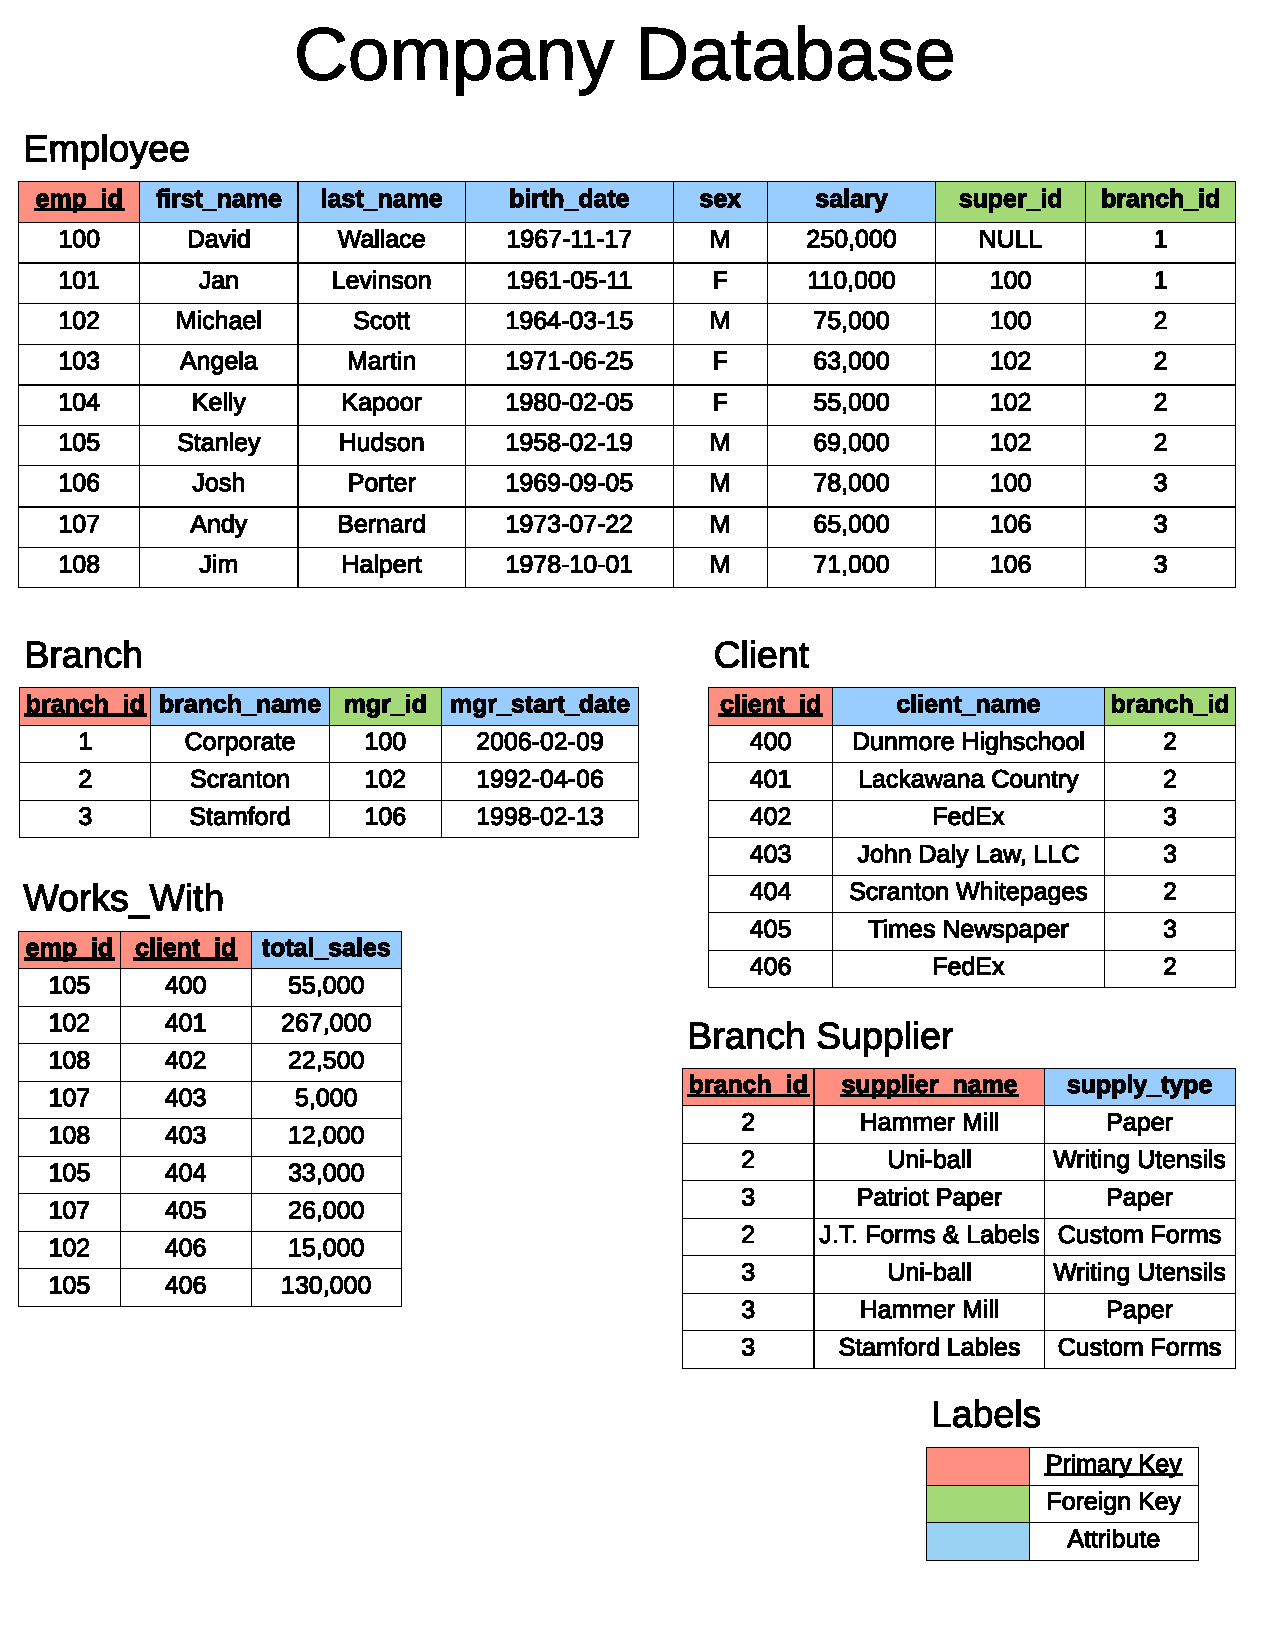
\includegraphics[width=0.7\textwidth]{Classes/company-database.pdf}
% 	\caption{}
\end{figure}


\section{Coding the schema of the company}
\begin{minted}[autogobble]{sql}
    use giraffe;
    create database giraffe;
    drop database giraffe;
    CREATE TABLE employee (
        emp_id INT PRIMARY KEY,
        first_name VARCHAR(40),
        last_name VARCHAR(40),
        birth_date DATE,
        sex VARCHAR(1),
        salary INT,
        super_id INT,
        branch_id INT
    );
    CREATE TABLE branch (
        branch_id INT PRIMARY KEY,
        branch_name VARCHAR(20), 
        mgr_id INT,
        mgr_start_date DATE,
        FOREIGN KEY(mgr_id) REFERENCES employee(emp_id) 
        ON DELETE SET NULL
    );

    -- Make employee.super_id and employee.branch_id foreign keys,
        -- we cannot do that just yet
    ALTER TABLE employee 
    ADD FOREIGN KEY(branch_id) 
    REFERENCES branch(branch_id) 
    ON DELETE SET NULL;

    ALTER TABLE employee 
    ADD FOREIGN KEY(super_id) 
    REFERENCES employee(emp_id) 
    ON DELETE SET NULL;

    CREATE TABLE client (
        client_id INT PRIMARY KEY,
        client_name VARCHAR(40),
        branch_id INT,
        FOREIGN KEY(branch_id) REFERENCES branch(branch_id) 
        ON DELETE SET NULL
    );
    CREATE TABLE works_with ( 
        emp_id INT,
        client_id INT,
        PRIMARY KEY(emp_id, client_id),
        FOREIGN KEY(emp_id) REFERENCES employee(emp_id) 
        ON DELETE CASCADE,
        FOREIGN KEY(client_id) REFERENCES client(client_id)
        ON DELETE CASCADE
    );
    CREATE TABLE branch_supplier (
        branch_id INT, 
        supplier_name VARCHAR(40),
        supply_type VARCHAR(40),
        PRIMARY KEY(branch_id, supplier_name),
        FOREIGN KEY(branch_id) REFERENCES branch(branch_id) 
        ON DELETE CASCADE
    );

    -- inserting the information
    -- Corporate branch.
    INSERT INTO employee VALUES(100,'David','Wallace','1967-11-17','M',350000,NULL,NULL);
    INSERT INTO branch VALUES(1,'Corporate',100,'2006-02-09');
    UPDATE employee SET branch_id = 1 WHERE emp_id = 100;
    INSERT INTO employee VALUES(101, 'Jan', 'Levinson', '1961-05-11','F',110000,100,1);

    -- Scranton branch.
    INSERT INTO employee VALUES(102, 'Michael', 'Scott', '1954-03-15','M',75000,100,NULL);
    INSERT INTO branch VALUES(2, 'Scranton',102,'1992-04-06');
    INSERT INTO employee VALUES(103, 'Angela', 'Martin', '1971-06-25','F',63000,102,2);
    INSERT INTO employee VALUES(104, 'Kelly', 'Kapoor', '1980-02-05','F',55000,102,2);
    INSERT INTO employee VALUES(105, 'Stanley', 'Hudson', '1958-02-19','M',69000,102,2);

    -- Stamford branch.
    INSERT INTO employee VALUES(106, 'Josh', 'Porter', '1959-09-05','M',78000,100,NULL);
    INSERT INTO branch VALUES(3, 'Scramford',106,'1998-02-13');
    UPDATE employee SET branch_id = 3 WHERE emp_id = 106;
    INSERT INTO employee VALUES(107,'Andy','Bernard','1973-07-22','M',65000,106,3);
    INSERT INTO employee VALUES(108,'Jim','Halpert','1978-10-01','M',71000,106,3);

    -- BRANCH SUPPLIER
    INSERT INTO branch_supplier VALUES(2,'Hammer Mill', 'Paper');
    INSERT INTO branch_supplier VALUES(2,'Uni-ball', 'Writing Utensil');
    INSERT INTO branch_supplier VALUES(3,'Patriot Paper', 'Paper');
    INSERT INTO branch_supplier VALUES(2,'J.T. Forms & Labels', 'Custom Forms');
    INSERT INTO branch_supplier VALUES(3,'Uni-ball', 'Writing Utensil');
    INSERT INTO branch_supplier VALUES(3,'Hammer Mill', 'Paper');
    INSERT INTO branch_supplier VALUES(3,'Stamford Lables', 'Custom Forms');

    -- WORKS WITH TABLE
    INSERT INTO works_with VALUES(105, 400, 55000);
    INSERT INTO works_with VALUES(102, 401, 267000);
    INSERT INTO works_with VALUES(108, 402, 22500);
    INSERT INTO works_with VALUES(107, 403, 5000);
    INSERT INTO works_with VALUES(108, 403, 12000);
    INSERT INTO works_with VALUES(105, 404, 33000);
    INSERT INTO works_with VALUES(107, 405, 26000);
    INSERT INTO works_with VALUES(102, 406, 15000);
    INSERT INTO works_with VALUES(105, 406, 130000);
\end{minted}
